\documentclass[main.tex]{subfiles}
\usepackage{util/estilo}

\begin{document}

Ejecutamos las pruebas en las siguientes máquinas, usando \texttt{fedora} como
la máquina para evaluar los solucionadores en CPU y \texttt{walle} como la
computadora para las pruebas en GPU.

\begin{verbatim}
Parameter,Value
Hostname,fedora
OS Info,"Fedora Linux 37 (KDE Plasma), Kernel: 6.5.12-100.fc37.x86_64"
glibc Version,2.36
CPU Model,AMD Ryzen 7 PRO 2700U w/ Radeon Vega Mobile Gfx
CPU Vendor,AuthenticAMD
CPU Flags,3dnowprefetch abm adx aes aperfmperf apic arat avic avx avx2 bmi1 bmi2 bpext clflush clflushopt clzero cmov cmp_legacy constant_tsc cpb cpuid cr8_legacy cx16 cx8 de decodeassists extapic extd_apicid f16c flushbyasid fma fpu fsgsbase fxsr fxsr_opt ht hw_pstate ibpb irperf lahf_lm lbrv lm mca mce misalignsse mmx mmxext monitor movbe msr mtrr mwaitx nonstop_tsc nopl npt nrip_save nx osvw overflow_recov pae pat pausefilter pclmulqdq pdpe1gb perfctr_core perfctr_llc perfctr_nb pfthreshold pge pni popcnt pse pse36 rapl rdrand rdseed rdtscp rep_good sep sev sev_es sha_ni skinit smap smca smep ssbd sse sse2 sse4_1 sse4_2 sse4a ssse3 succor svm svm_lock syscall tce topoext tsc tsc_scale v_vmsave_vmload vgif vmcb_clean vme vmmcall wdt xgetbv1 xsave xsavec xsaveerptr xsaveopt
Logical Cores,8
Physical Cores,4
Base Frequency (MHz),1600.0
Boost Frequency (MHz),2200.0
Chipset,83DA
L1d Cache,128 KiB (4 instances)
L1i Cache,256 KiB (4 instances)
L2 Cache,2 MiB (4 instances)
L3 Cache,4 MiB (1 instance)
OpenMP Version,4.5
Total RAM (GB),14.55
CUDA Capable Device,N/A
CUDA Version,N/A
AVX Supported,Yes
SSE Supported,Yes
\end{verbatim}

\begin{verbatim}
Parameter,Value
Hostname,WallE
OS Info,"Ubuntu 22.04.5 LTS, Kernel: 5.15.167.4-microsoft-standard-WSL2"
glibc Version,2.35
CPU Model,AMD Ryzen 5 2600 Six-Core Processor
CPU Vendor,AuthenticAMD
CPU Flags,3dnowprefetch abm adx aes apic arat avx avx2 bmi1 bmi2 clflush clflushopt clzero cmov cmp_legacy constant_tsc cpuid cr8_legacy cx16 cx8 de decodeassists extd_apicid f16c flushbyasid fma fpu fsgsbase fxsr fxsr_opt ht hypervisor ibpb lahf_lm lm mca mce misalignsse mmx mmxext movbe msr mtrr nonstop_tsc nopl npt nrip_save nx osvw osxsave pae pat pausefilter pclmulqdq pdpe1gb perfctr_core pfthreshold pge pni popcnt pse pse36 rdrand rdrnd rdseed rdtscp rep_good sep sha sha_ni smap smep ssbd sse sse2 sse4_1 sse4_2 sse4a ssse3 svm syscall topoext tsc tsc_reliable tsc_scale v_vmsave_vmload virt_ssbd vmcb_clean vme vmmcall xgetbv1 xsave xsavec xsaveerptr xsaveopt
Logical Cores,12
Physical Cores,6
Base Frequency (MHz),3.2
Boost Frequency (MHz),3.7
Chipset,N/A
L1d Cache,192 KiB (6 instances)
L1i Cache,384 KiB (6 instances)
L2 Cache,3 MiB (6 instances)
L3 Cache,8 MiB (1 instance)
OpenMP Version,4.5
Total RAM (GB),15.60
CUDA Capable Device,Yes
NVIDIA GPU Model,NVIDIA GeForce GTX 1060 6GB
Global Memory,6.00 GB
Shared Memory per Block,49152 bytes
Warp Size,32
Streaming Multiprocessor Count,20
Compute Capability,6.1
CUDA Core Count,1280
PCIe Bus Bandwidth,<15.76GB
GPU Memory Bus Width, 192-bit
CUDA Version,12.5
AVX Supported,Yes
SSE Supported,Yes
\end{verbatim}

Escogimos las siguientes instancias de TSPLIB95 pues sus tamaños nos parecieron
relevantes, pero no ejecutamos todos los problemas con todos los solucionadores
pues el tiempo de cómputo lo prohibía por limitaciones de tiempo en cuanto a la
realización del proyecto.

Los datos de las ejecuciones resumidas se pueden revisar lanzando el notebook
de Jupyter.

Teniendo instalado \texttt{pip} y \texttt{python3}, basta con estar sobre el
directorio \mbox{\texttt{/analysis}} y ejecutar \mbox{\texttt{./launch}}. Ahí
mismo se realiza una pequeña discusión a manera de análisis de los resultados.

Para evitar duplicar toda la información del notebook, en este reporte
dejaremos algunos datos importantes e interesantes de lado, y nos enfocaremos
únicamente en los resultados de tiempos de ejecución. Recomendamos explorar el
notebook con mayor detalle para ver los resultados completos.

\begin{cajaEnunciado}
    \addcontentsline{toc}{subsubsection}{Máximo Esfuerzo GPU}
    \textbf{Máximo esfuerzo GPU}
\end{cajaEnunciado}

\begin{center}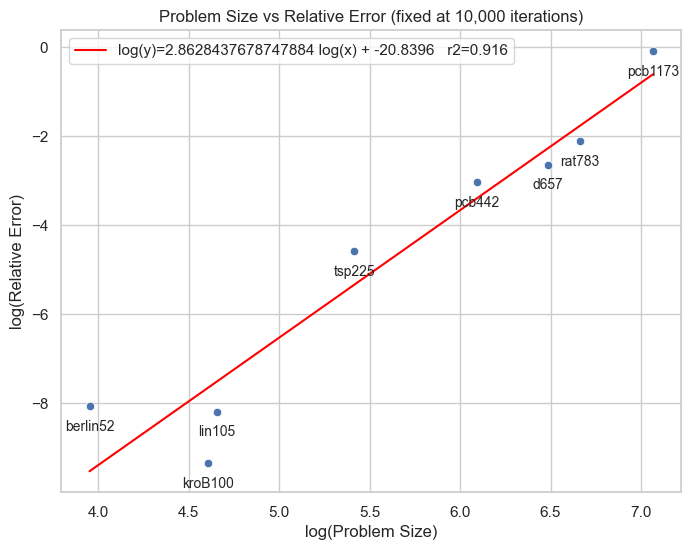
\includegraphics[width=3.5in]{MaxEffort1.png} 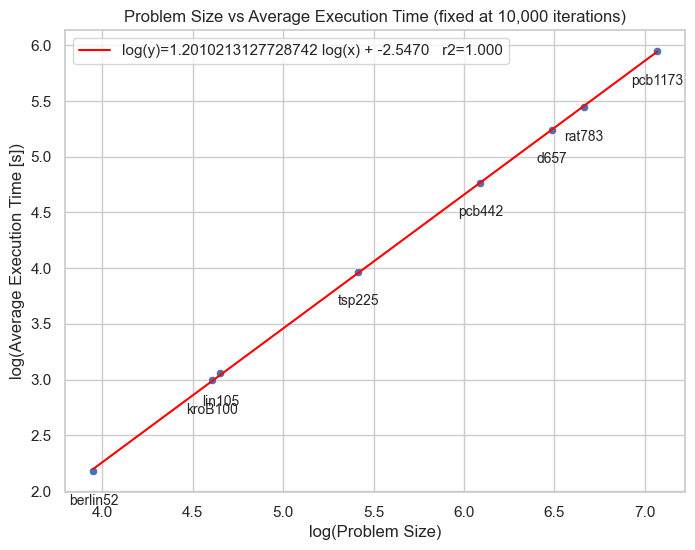
\includegraphics[width=3.5in]{MaxEffort2.png}\end{center}

\begin{center}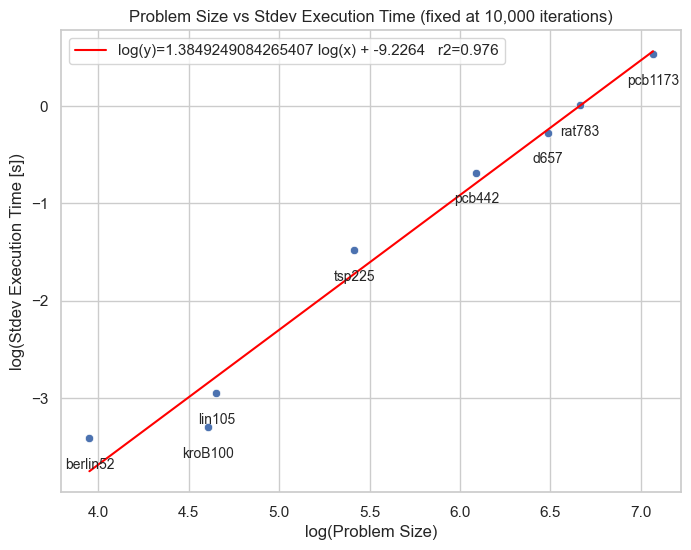
\includegraphics[width=3.5in]{MaxEffort3.png} 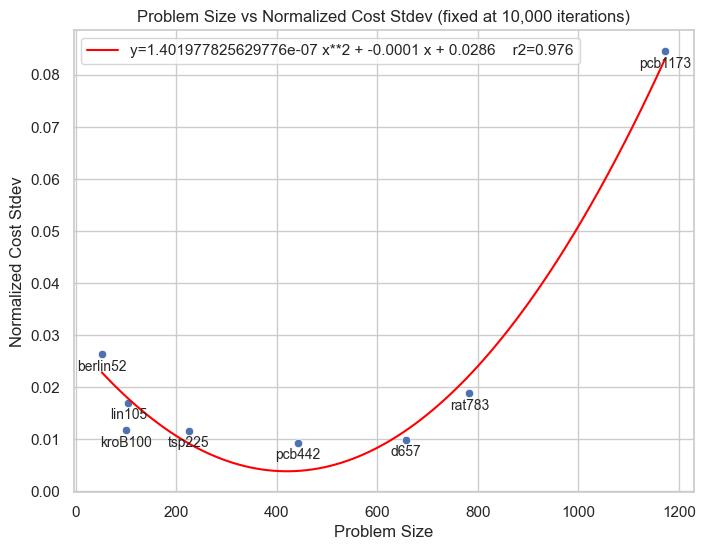
\includegraphics[width=3.5in]{MaxEffort4.png}\end{center}

\begin{cajaEnunciado}
    \addcontentsline{toc}{subsubsection}{Punto de Corte}
    \textbf{Punto de Corte}
\end{cajaEnunciado}

\begin{center}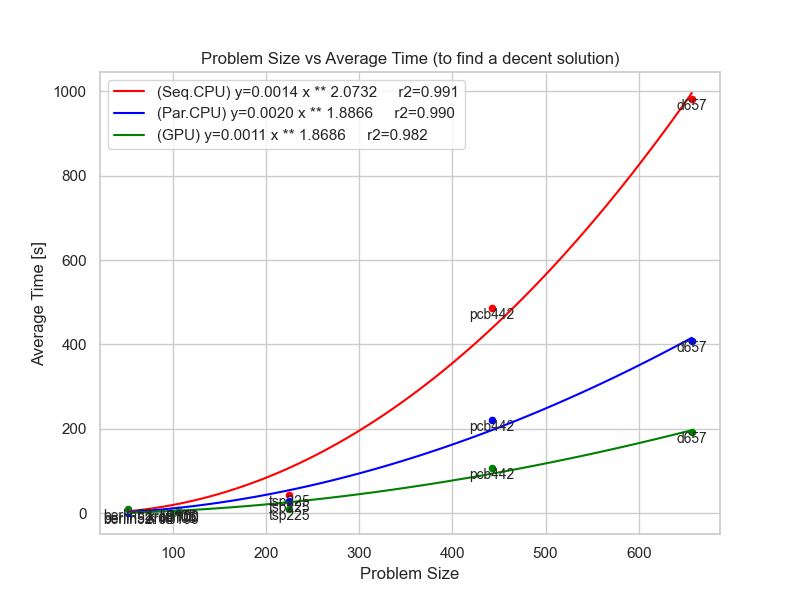
\includegraphics[width=3.5in]{Cutoff1.png} 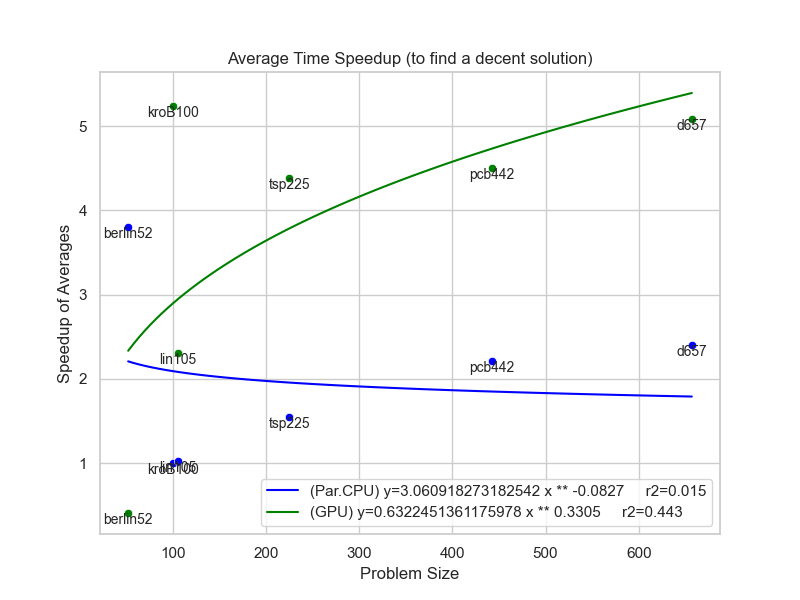
\includegraphics[width=3.5in]{Cutoff2.png}\end{center}

\begin{center}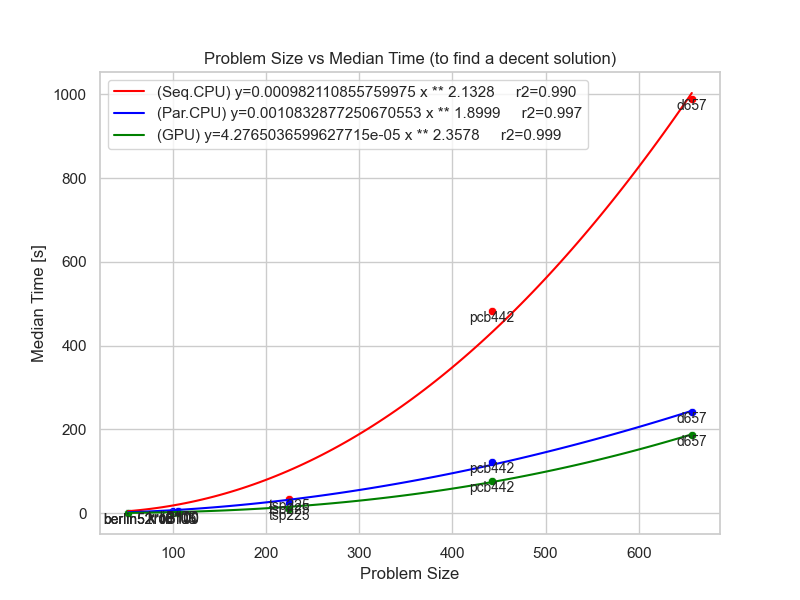
\includegraphics[width=3.5in]{Cutoff3.png} 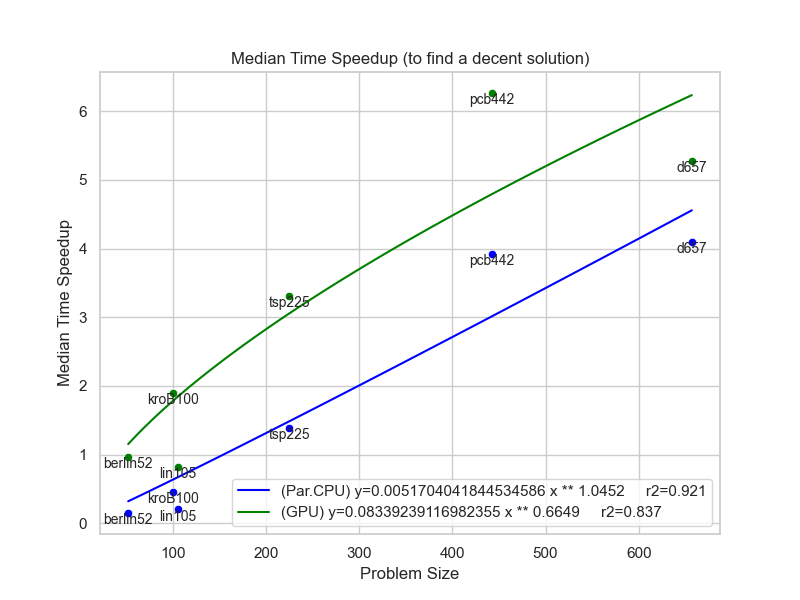
\includegraphics[width=3.5in]{Cutoff4.png}\end{center}

\begin{center}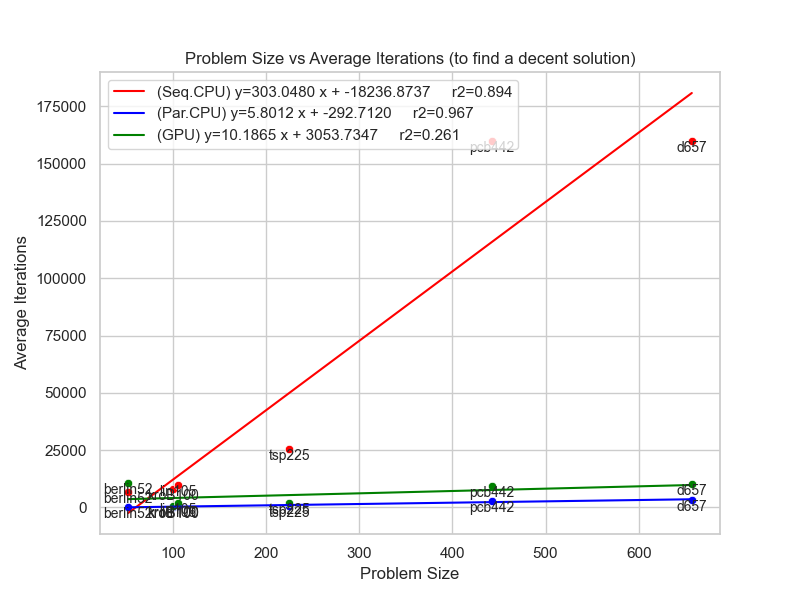
\includegraphics[width=3.5in]{Cutoff5.png} 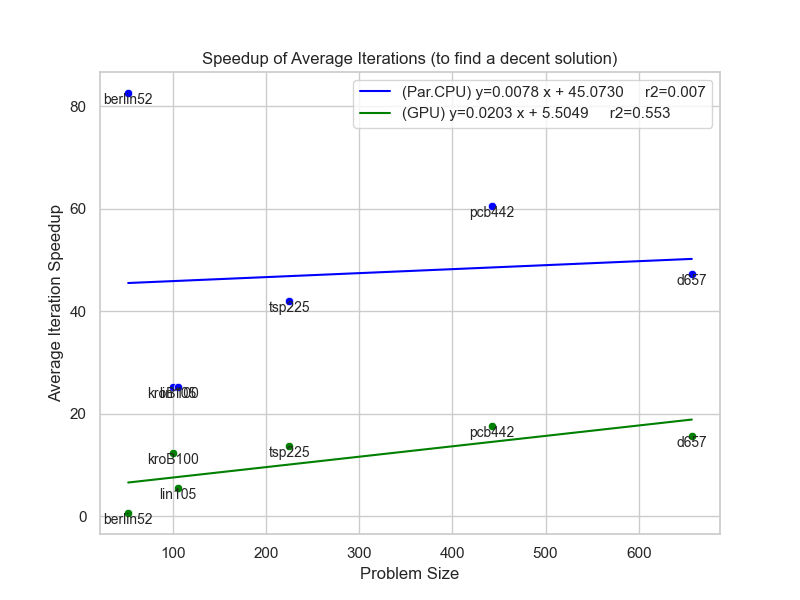
\includegraphics[width=3.5in]{Cutoff6.png}\end{center}

\begin{center}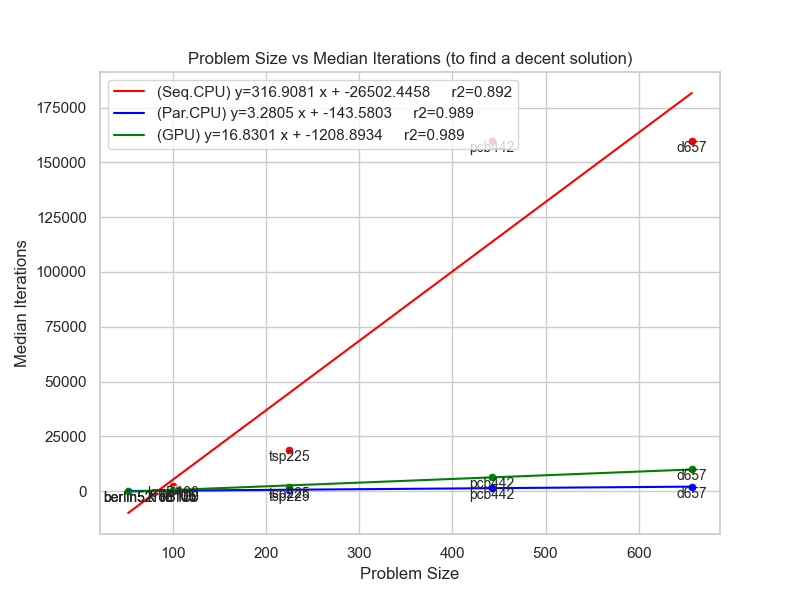
\includegraphics[width=3.5in]{Cutoff7.png} 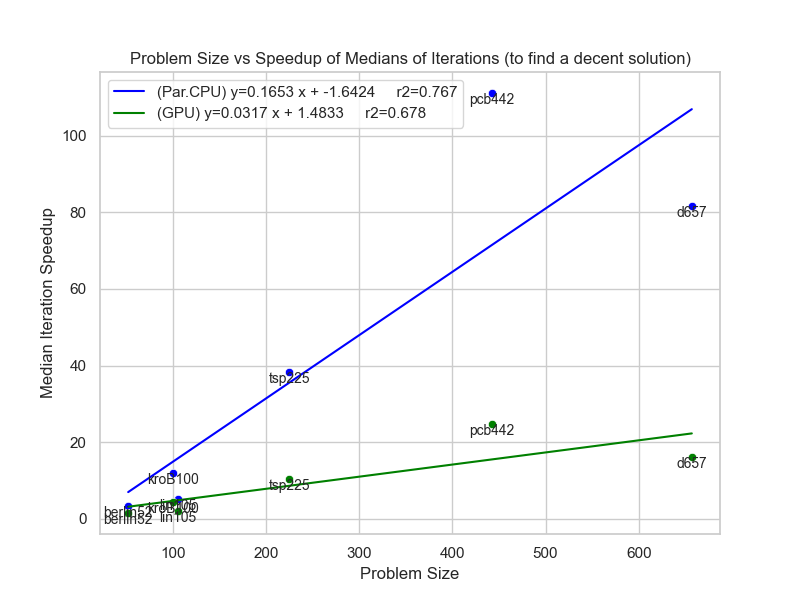
\includegraphics[width=3.5in]{Cutoff8.png}\end{center}

\end{document}

